\documentclass[12pt,twocolumn]{article}
\usepackage[margin=1.5cm]{geometry}
\usepackage{amsmath}
\usepackage{graphicx}
\usepackage{hyperref}
\usepackage{sectsty}
\title{Study Guide for Midterm 2}
\author{Prof. Jordan C. Hanson}
\sectionfont{\fontsize{12}{15}\selectfont}

\begin{document}
\maketitle
\small

\section{Unit 4: Magnetism II}

\begin{figure}
\centering
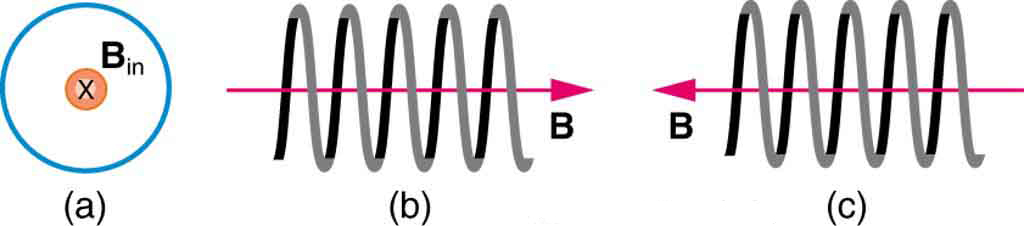
\includegraphics[width=0.4\textwidth]{b-field_1.jpeg}
\caption{\label{fig:B-flux} \small (a) A current $I$ flows in a loop. (b) A coil of wire with current $I$ flows.  (c) A coil of wire with current $I$ flows.}
\end{figure}

\noindent
\begin{enumerate}
\item Consider Fig. \ref{fig:B-flux} (a)-(c).  (a) What is the direction of the current $I$ in Fig. \ref{fig:B-flux} (a)?  (b) What is the direction of the current $I$ in Fig. \ref{fig:B-flux} (b)?  (c) What is the direction of the current $I$ in Fig. \ref{fig:B-flux} (c)? \\ \vspace{2cm}
\item (a) An MRI technician moves his hand from a region of very low magnetic field strength into an MRI scanner's 0.75 T field with his fingers pointing in the direction of the field. Find the average emf induced in his wedding ring, given its diameter is 1.2 cm and assuming it takes 50 ms to move it into the field. (b) What current is induced in the ring if its resistance is 0.05 $\Omega$? \\ \vspace{2cm}
\item The \textbf{Hall Effect} occurs when a current-carrying conductor transports charges in a direction perpendicular to a B-field.  Negative and positive charge separate until a voltage appears across the conductor.  The voltage corresponds to an E-field that balances the force on additional charge that moves through the B-field.  (a) Show that if the net force on positive charges in current is zero, that the Hall voltage is $\Delta V_{\rm H} = B l v$, where $l$ is the width of the conductor, and $v$ is the speed of the positive charges.  (b) Given the definition of current in terms of \textit{drift velocity}, show that $\Delta V_{\rm H}$ is proportional to current.  \\ \vspace{3cm}
\item (a) What is the peak voltage of a generator rotating at 1000 rad/s, if it is assembled from $N = 100$ coils of wire that form a loop with area 0.1 m$^2$ in a 0.5 T B-field? \\ \vspace{2cm}
\item Imagine you are traveling to a country in Latin America that does not use the American 120 V system for wall power.  (a) Design a small transformer that converts 180 V AC power to our 120 V AC power, by choosing the correct ratio of turns in the transformer input and output coils. (b) If we power a device that requires 50 W at 120 V AC, what current will occur on the transformer input? \\ \vspace{2cm}
\item If we charge a 0.1 mH inductor by turning on a 1.0 Amp current in 10 ms, (a) what is the induced emf? (b) What is the stored energy? (c) Design a solenoid that acts as an inductor with 0.1 mH. \\ \vspace{2cm}
\item Your RL circuit has a characteristic time constant of 100.0 ns, and a resistance of 0.5 M$\Omega$. (a) What is the inductance of the circuit? (b) Scaling problem: what resistance would give you a 200.0 ns time constant? (c) What is the reactance of the inductor at 1 kHz? \\ \vspace{2cm}
\item Consider Fig. \ref{fig:RC}.  (a) Model this circuit in the AC circuits PhET, and graph the ratio $v_{\rm out}/v_{\rm in}$. (b) Is this a low-pass or high-pass filter? \\ \vspace{3cm}
\item (a) What are the resonance frequency, $f_0$, and resonance width, $\Delta f/f_0$, of an RLC circuit with $R = 10$ $\Omega$, $C = 10$ $\mu$F, and $L = 100$ mH? (b) What is the total impedance of this circuit at twice the resonance frequency? (c) What is the rms current, if the rms voltage at this frequency is 120 V? \\ \vspace{1.5cm}
\item Suppose we are using an LC resonator and diode combination to create an AM radio signal.  If the resonance frequency of our resonator is 0.740 MHz, and our audio signal is at 5 kHz, what three frequencies should be present in our AM radio spectrum? \\ \vspace{1cm}
\end{enumerate}

\begin{figure}
\centering
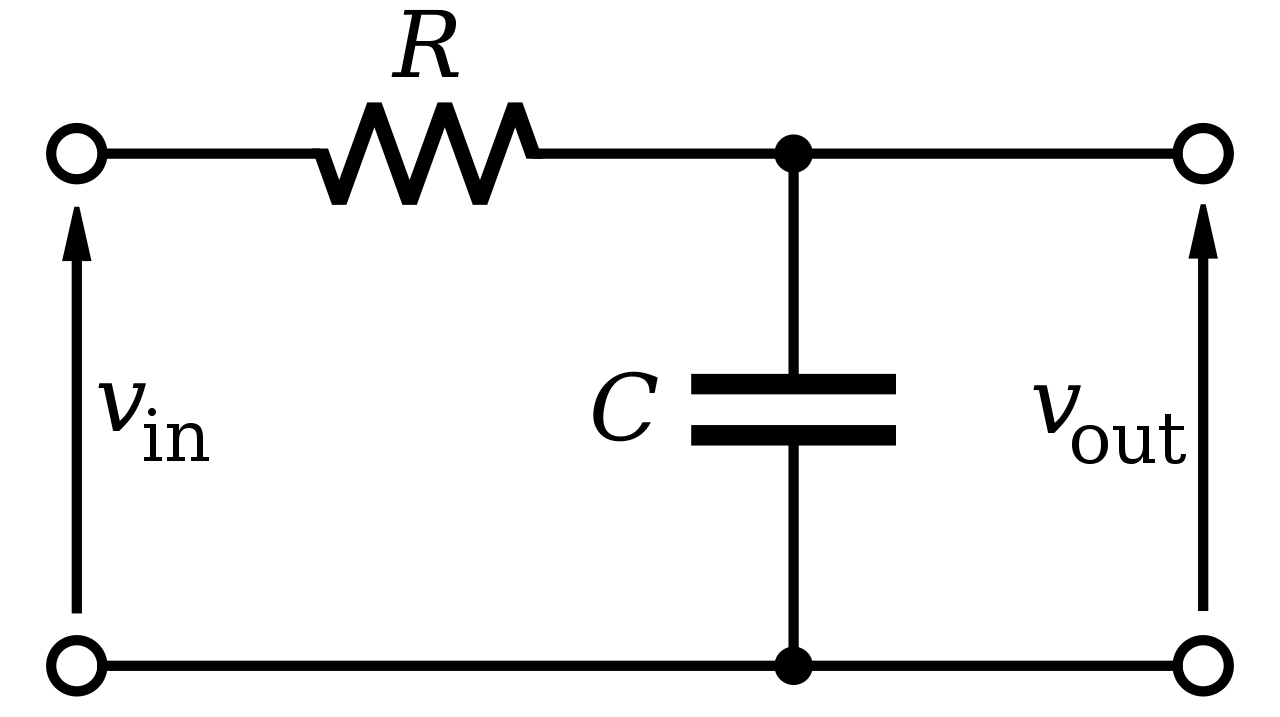
\includegraphics[width=0.25\textwidth]{low-pass.png}
\caption{\label{fig:RC} \small This RC circuit can act as a filter.}
\end{figure}

\section{Unit 5: Waves, Optics, Medical Physics}

\begin{figure}
\centering
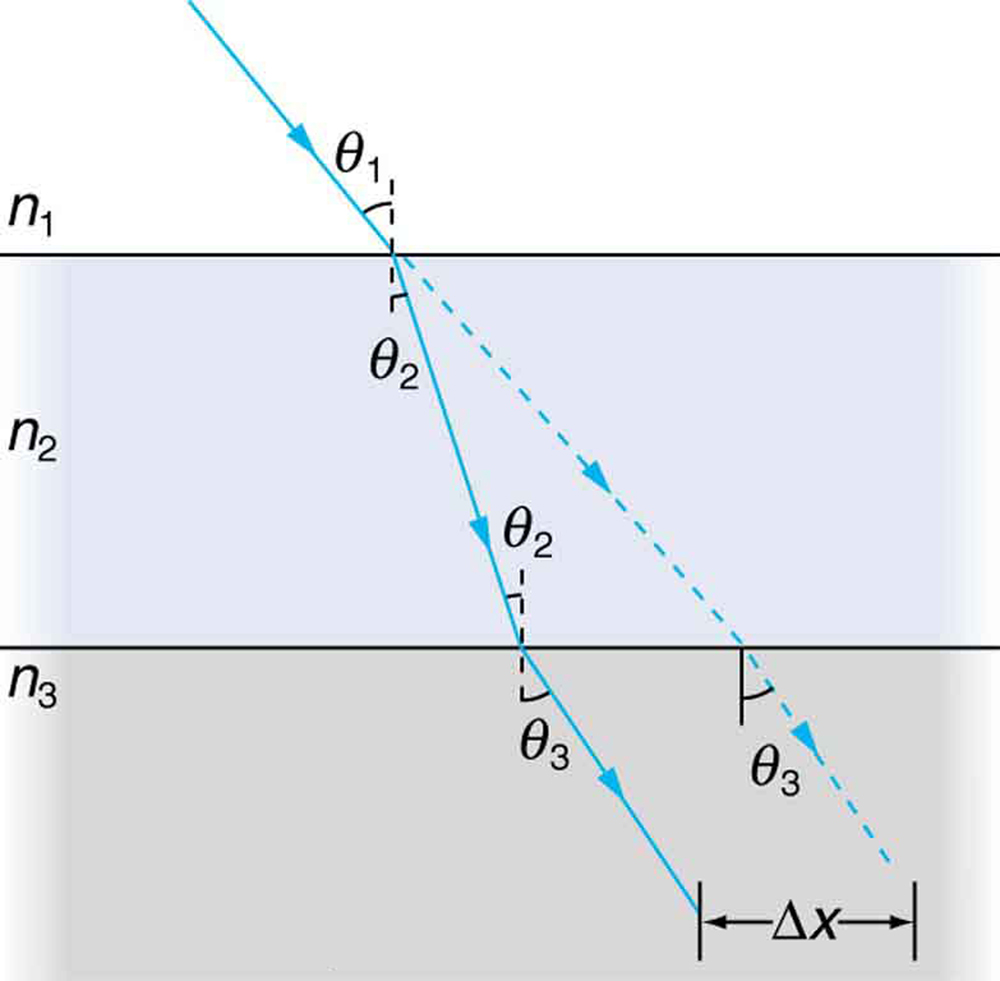
\includegraphics[width=0.25\textwidth]{lens_1.jpeg}
\caption{\label{fig:lens_1} \small A light ray is in a medium with $n_1$, then enters a medium with $n_2$, then a medium with $n_3$.}
\end{figure}

\noindent
\begin{enumerate}
\item (a) What is the B-field generated 0.1 cm laterally from a capacitor in an RC circuit that charges from 0 to 500 nC in 1 $\mu$s? (b) What \textit{current} is responsible for this B-field? \\ \vspace{2cm}
\item (a) An aircraft receives a pulse reflected from glacial ice below it $5$ $\mu$s after transmission. What is the displacement between aircraft and ice? (b) What fraction of the radar power is reflected from the ice, assuming normal incidence? \\ \vspace{2.5cm}
\item (a) A microwave generates 0.5 kW of power, projected onto a 400 cm-squared area at a distance of 1 m.  What is the intensity (power per unit area)? (b) What is the peak E-field at the source? \\ \vspace{2.5cm}
\item Consider Fig. \ref{fig:lens_1}.  (a) If $n_1 = 1.0$, and $n_2 = 1.3$, and $\theta_1 = 30$ degrees, what is $\theta_2$? \\ \vspace{2cm}
\item Analysis of an interference effect in a clear solid shows that the wavelength of light in the solid is 329 nm. Knowing this light comes from a He-Ne laser and has a wavelength of 633 nm in air, is the substance zircon or diamond?  \\ \vspace{1cm}
\item Suppose x-rays have a cross section of 150 barns at 5 keV in a lead vest protecting a medical patient. (a) If the vest is 0.5 cm thick, what fraction of the x-rays pass through it? \\ \vspace{2cm}
\item Some nuclear isotopes emit \textit{free neutrons}, neutrons that then propagate outside the nucleus.  These neutrons are useful for controlling nuclear fission for power production, and have a half-life of $611\pm 1$ seconds in free space.  (a) If emitted in free space, what fraction of the neutrons remain after 12 hours? \\ \vspace{1cm}
\item (a) What is the radioactive dose in rads if 125 mJ of total energy is deposited in the body of a 80 kg adult? (b) What instead would be the dose if the radiation was concentrated in just 1.0 kg of tissue? \\ \vspace{2cm}
\end{enumerate}

\end{document}